\subsection{\ac{ADCS}}
\label{mtrTOpruneadcs}
Gravity-gradient stabilisation and passive magnetic are eliminated as options, because they are not accurate enough and they do not allow pointing to a specific ground target other than the mass or magnetic centre of the Earth. Spin stabilisation is pruned, because the satellite needs to be able to make measurements continuously. Double gimbal \acp{CMG} are also not a viable option, because they are to complex and heavy compared to the other systems.
For the attitude determination initial measurements and magnetometers are found not to be good enough, because of their low accuracy over time.
The pruned design option tree can be found in figure \ref{fig:mtrTOpruneadcs} on page \pageref{fig:mtrTOpruneadcs}.

\begin{figure}
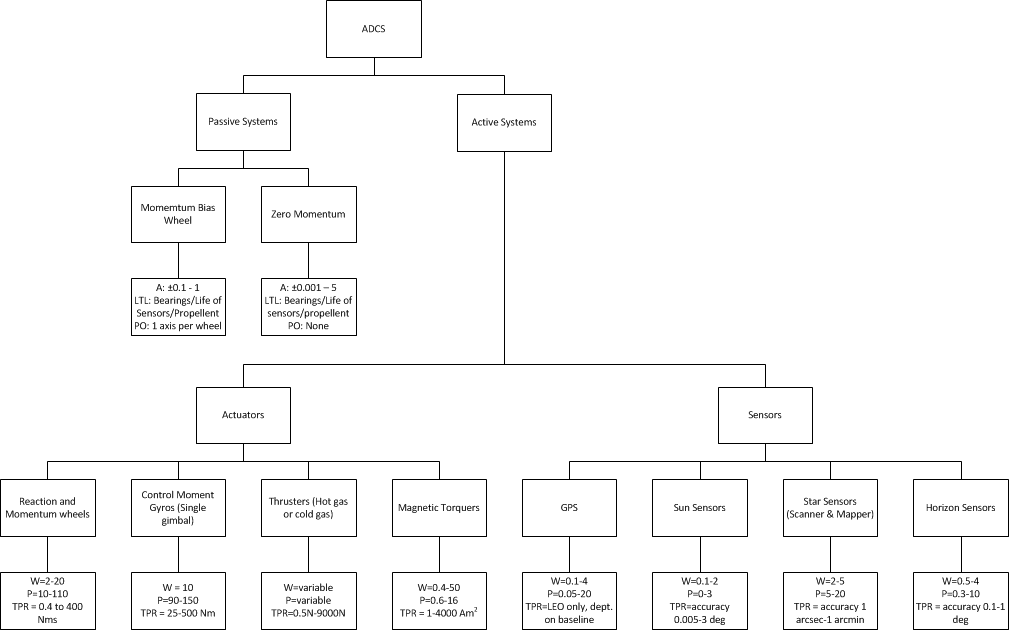
\includegraphics[width=0.8\textwidth, angle=90]{chapters/MTR/img/prunedADCStree.png}
\label{fig:mtrTOpruneadcs}
\caption{Pruned design option tree for \ac{ADCS}}
\end{figure}